\chapter{Inter-Process Communication}
\section{Introduction}
Processes in a distributed system require the ability to communicate with each other; this is called Inter-Process Communication (IPC). There are two basic approaches underlying IPC (as can be seen in \autoref{fig:screenshot009}):
\begin{itemize}
\item \textbf{Original sharing}: there is a shared memory area, and both processes access it.
\item \textbf{Copy sharing}: messages are sent between the processes through some mechanism, and no memory is shared to facilitate this.
\end{itemize}

\begin{figure}[h]
\centering
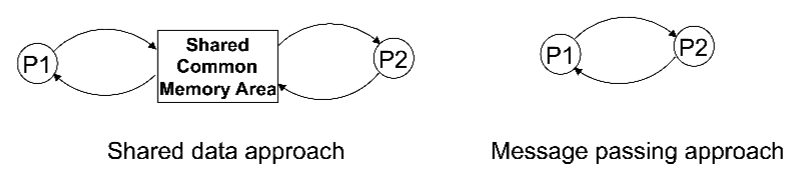
\includegraphics[width=0.7\linewidth]{figures/screenshot009}
\caption{Comparison of approaches to IPC}
\label{fig:screenshot009}
\end{figure}

A \textit{message-passing system} is a component of a distributed system that provides a message-based IPC system for the rest of the system. In doing so, it abstracts away the details of the underlying network protocols and heterogeneous computing platforms.

Processes can communicate by exchanging messages; these messages are transferred using simple primitives such as \texttt{send} and \texttt{receive}.

Higher-level IPC systems, such as Remote Procedure Call (RPC) and Distributed Shared Memory (DSM), can be built on top of a message-passing system.

\section{Design Constraints}
A "good" message-passing system will generally have the following features:
\begin{itemize}
\item \textbf{Simplicity}
\item \textbf{Uniform semantics}: The same primitives are used for both local and remote communication
\item \textbf{Efficiency}: The system should aim to reduce the number of messages where possible, and make each message as efficient as possible. Ways to accomplish this include: \begin{itemize}
	\item Avoiding the cost of establishing and terminating connections between a pair of processes for every new message between them
	\item Minimising the cost of maintaining a connection
	\item Bundling an acknowledgement of a previous message and a response together
\end{itemize}
\item \textbf{Reliability}: The system should handle lost and duplicated messages reliably.
\item \textbf{Correctness}: The system should obey the following properties: \begin{enumerate}
	\item \textbf{Atomicity}
	\item \textbf{Ordered delivery}
	\item \textbf{Survivability}
\end{enumerate}
\item \textbf{Flexibility}: Not all systems require the full suite of correctness properties. A system should be able to disable one or more of these properties in exchange for better performance or improvement along some other metric.
\item \textbf{Security}: The sender and receiver of a message should be authenticated, and there should be facilities for encrypting a message.
\item \textbf{Portability}: The message-passing system should be portable (i.e. deployable across a wide variety of platforms); similarly, applications using IPC protocol primitives should also be portable.
\end{itemize}

The structure of a typical message in a message-passing system may look something like this:
\begin{itemize}
\item Header \begin{itemize}
	\item Addresses \begin{itemize}
		\item Sender address
		\item Receiver address
	\end{itemize}
	\item Sequence number
	\item Structural information \begin{itemize}
		\item Type
		\item Number of bytes
	\end{itemize}
	\end{itemize}
\item Message
\end{itemize}

Issues that need to be considered while designing an IPC protocol include:
\begin{itemize}
\item \textbf{Identity}: Who is the sender? Who is the receiver?
\item \textbf{Network Topology}: Is there one receiver for a message, or many? If so, how do you handle this?
\item \textbf{Flow control}: Is acknowledgement of a message guaranteed by the receiver? Should the sender wait for acknowledgement?
\item \textbf{Error control and channel management}: What happens if a node crashes? What happens if the receiver's not ready? How does a node deal with multiple outstanding messages?
\end{itemize}

\section{Synchronisation}
As processes run independently, they must synchronise in order to communicate. To do this, their send/receive primitives can operate in one of two modes: blocking, or non-blocking.

When using blocking semantics, the primitive will halt execution of the program until the operation has terminated. In the case of a send, this may mean that execution will be blocked until either the message has been sent or until it has been acknowledged by the receiving party. In the case of a receive, this means that execution will halt until a message is received.

When using non-blocking semantics, the program will attempt to complete the operation, but program execution will not be halted. The status of an operation can be checked to determine whether an operation has completed. This allows operations to be interleaved with work, which increases efficiency. A non-blocking send will queue up a message send with the operating system, and will then exit. A non-blocking receive will attempt to receive the data, but will do nothing if there is no message or if the data cannot be received yet.

When both sending and receiving of a communication between processes is blocking, the communication is \textit{synchronous}; otherwise, it is \textit{asynchronous}. A synchronous workflow can be seen in \autoref{fig:screenshot010}.

\begin{figure}[h]
\centering
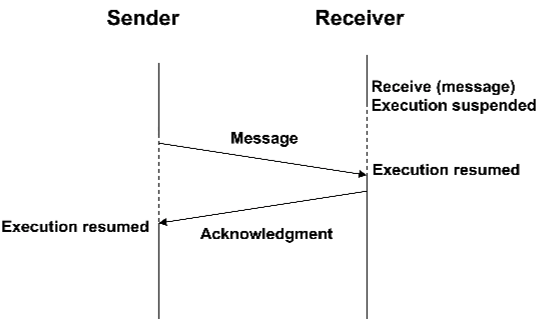
\includegraphics[width=0.4\linewidth]{figures/screenshot010}
\caption{Synchronous workflow for send/receive}
\label{fig:screenshot010}
\end{figure}

Advantages of synchronous communication include \begin{itemize}
\item being simple and easy to implement
\item increased reliability
\item not requiring backward error recovery
\end{itemize}

Advantages of asynchronous communication include \begin{itemize}
\item high concurrency
\item being more flexible than synchronous communication
\item having a lower deadlock risk than synchronous communication (but not impossible!)
\end{itemize}

A synchronous system uses no buffer for sending, and a single buffer for receiving. An asynchronous system uses an unbounded capacity buffer for both sending and receiving where the buffer can contain multiple messages. This can be seen in \autoref{fig:screenshot011}.

\begin{figure}[h]
\centering
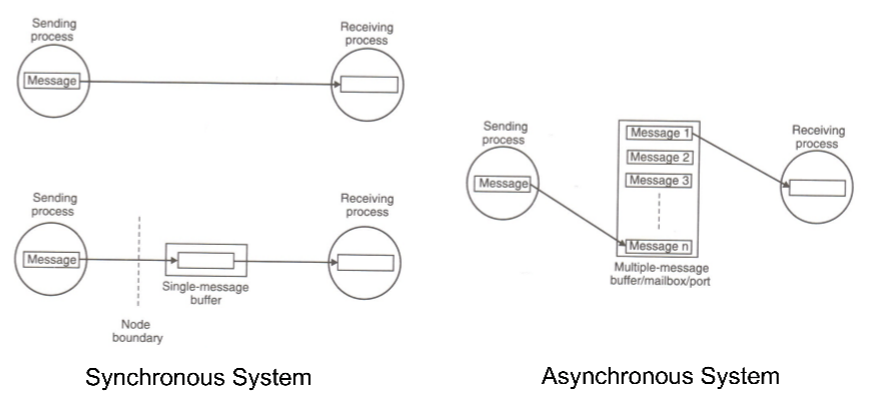
\includegraphics[width=0.9\linewidth]{figures/screenshot011}
\caption{Buffering in a synchronous system versus an asynchronous system}
\label{fig:screenshot011}
\end{figure}

\section{Message Delivery Concerns}
\subsection{Multi-datagram messages}
Almost all networks have an upper bound on the size of data that can be transferred in a single message; this quantity is known as the \textit{MTU} (maximum transfer unit).

A message with a size greater than the MTU must be split apart (\textit{fragmented}) into multiple packets, each of which is called a \textit{datagram}.

Messages can thus be classified as a \textit{single-datagram message} or a \textit{multi-datagram message}. Disassembly and re-assembly of a multi-datagram message is the responsibility of a message-passing system.

A potential algorithm for re-assembly of a multi-datagram message is shown in \autoref{fig:screenshot012}. It uses a \textit{bitmap} to represent each datagram of the packet. When a datagram comes in, the corresponding bit in the bitmap is set. If the last datagram of a message arrives and the message is not complete, a request for the missing datagrams is sent to the sender. When all bits are set and the message can be reconstructed, an acknowledgement is sent to the sender.

\begin{figure}[h]
\centering
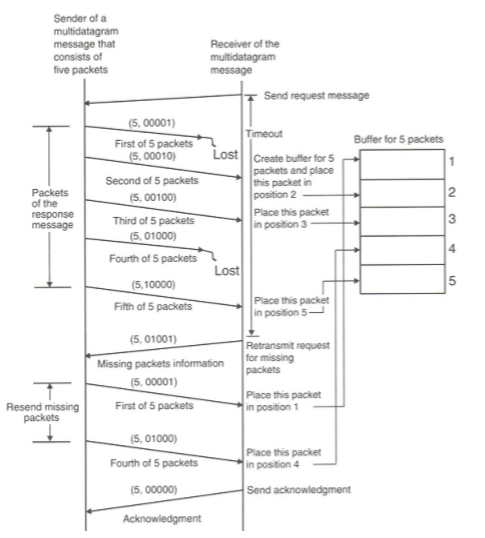
\includegraphics[width=0.4\linewidth]{figures/screenshot012}
\caption{Bitmap algorithm for multi-datagram message reconstruction}
\label{fig:screenshot012}
\end{figure}

\subsection{Encoding/Decoding}
Encoding and decoding are required if the sender and the receiver have a different computing architecture. However, it may still be required if the message to be sent uses an absolute pointer to memory on the sender's machine, or if the message contains a user-defined object that the receiver does not necessarily know how to identify.

\subsection{Process Addressing}
When sending or receiving a message, explicit or implicit addressing can be used. Explicit addressing requires a specific process ID to send to or receive from, while implicit addressing requires the ID of a \textit{service} (a group of processes belonging to a particular use-case \footnote{I don't know if this is actually correct. I'm guessing based on my use of MPI, but the slides don't go into detail on this.}) to send to or receive from.

\subsection{Failure Handling}
There are three kinds of failure that can potentially occur in a message-passing system: the request could be lost, the response could be lost, or the request may have failed to execute on the receiver side. These are illustrated in \autoref{fig:screenshot013}.

\begin{figure}[h]
\centering
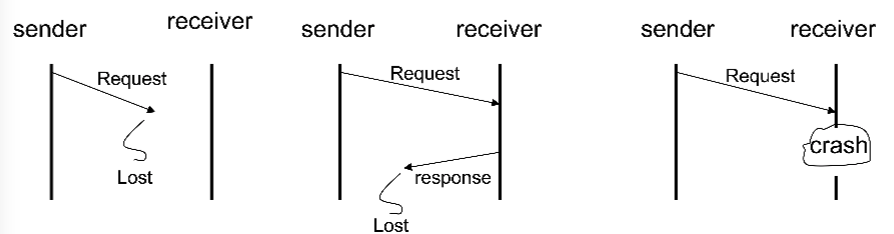
\includegraphics[width=0.6\linewidth]{figures/screenshot013}
\caption{Potential failures in a message-passing system.}
\label{fig:screenshot013}
\end{figure}

The following diagrams illustrate "reliable" IPC protocols to accommodate failure. However, one side may end up blocked indefinitely \footnote{Unless a timeout is used to terminate the blocking operation after some time. This is not mentioned in the slides, but it is the obvious way to make these at least \textit{somewhat} realistic.} ; these protocols do not illustrate intelligent re-send/waiting behaviour.

\begin{tabular}{|c|c|c|}
\hline 
\multicolumn{3}{|c|}{Number of messages}  \\ 
\hline 
4 & 3 & 2 \\ 
\hline 
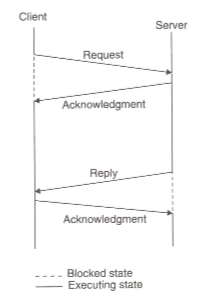
\includegraphics[width=0.3\linewidth, trim=0 0 0 -5]{figures/screenshot014}
 & 
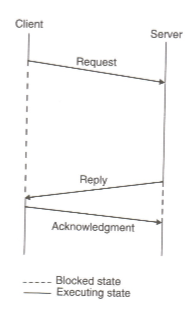
\includegraphics[width=0.3\linewidth, trim=0 0 0 -5]{figures/screenshot015}
 & 
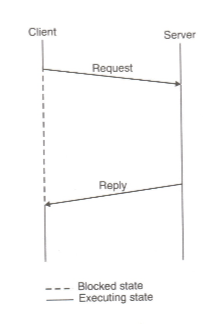
\includegraphics[width=0.3\linewidth, trim=0 0 0 -5]{figures/screenshot016}
  \\ 
\hline 
\end{tabular} 

An example of a fault-tolerant system is shown in \autoref{fig:screenshot017}. Note how the system deals with request loss, request execution failure, and loss of execution. The second execution of the request may result in different behaviour; this is covered in \autoref{ssec:idempotency}.

\begin{figure}[h]
\centering
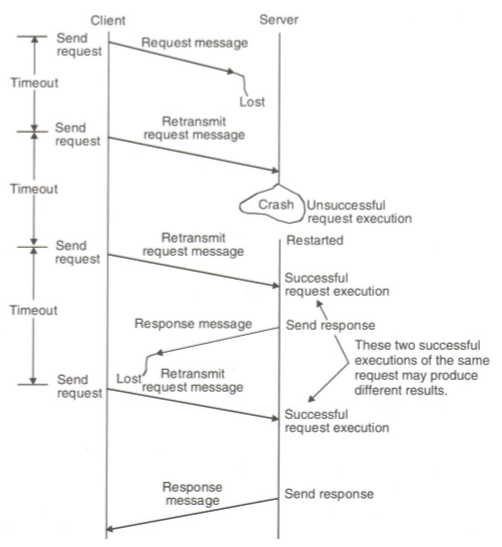
\includegraphics[width=0.4\linewidth]{figures/screenshot017}
\caption{An example of a fault-tolerant system.}
\label{fig:screenshot017}
\end{figure}

\subsection{Idempotency}
\label{ssec:idempotency}
An idempotent function will return the same result given the same input, even when executed multiple times. For example, an idempotent function is illustrated in \autoref{alg:idempotent}; a non-idempotent function is illustrated in \autoref{alg:nonidempotent}.

\begin{algorithm}
\caption{An example of an idempotent function.}
\label{alg:idempotent}
\begin{algorithmic}
\Function{getSqrt}{n}
	\State \Return \Call{sqrt}{n}
\EndFunction
\end{algorithmic}
\end{algorithm}

\begin{algorithm}
\caption[Example of a non-idempotent function]{An example of a non-idempotent function. This function will return different values when given the same input. An illustration of the flow can be seen in \autoref{fig:screenshot018}.}
\label{alg:nonidempotent}
\begin{algorithmic}
\Function{debit}{amount}
	\If {balance $>$ amount}
		\State balance $\gets$ balance $-$ amount
		\State \Return ("success", balance)
	\Else
		\State \Return ("failure", balance)
	\EndIf
\EndFunction
\end{algorithmic}
\end{algorithm}

\begin{figure}[h]
\centering
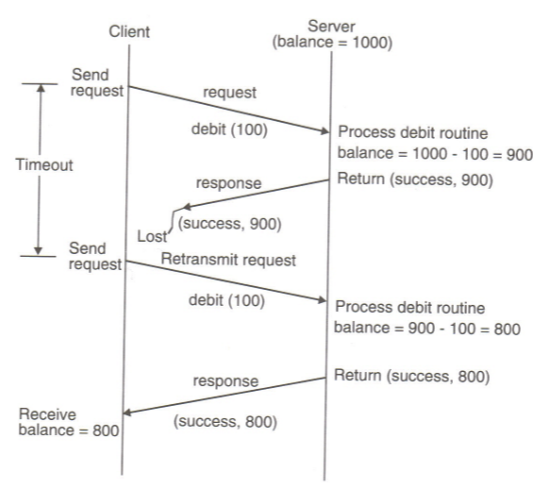
\includegraphics[width=0.55\linewidth]{figures/screenshot018}
\caption{Non-idempotent function in a distributed system.}
\label{fig:screenshot018}
\end{figure}

To mitigate the effects of non-idempotent functionality in a distributed system, a layer can be implemented on top of a non-idempotent function to make it appear idempotent. This can be done by adding a sequence number for the request message, and then adding a \textit{reply cache} that stores response for a sequence number.

When a request is handled by a receiver, the response is stored in the reply cache and is indexed by the sequence number. If the request is re-received (i.e. as the sender failed to receive the response), the reply cache will return the saved response instead of running the non-idempotent operation again. This is illustrated in \autoref{fig:screenshot019}.

\begin{figure}
\centering
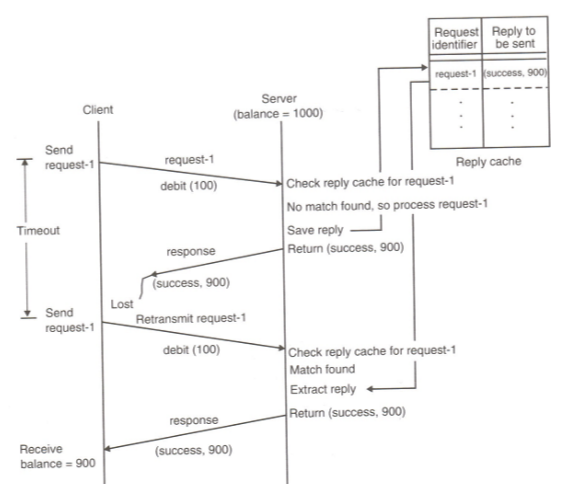
\includegraphics[width=0.7\linewidth]{figures/screenshot019}
\caption[Non-idempotent to idempotent using reply cache]{Conversion of a non-idempotent operation to an idempotent operation using a reply cache.}
\label{fig:screenshot019}
\end{figure}

\section{Group Communication}
Group communication may involve one-to-many, many-to-one, and many-to-many communication.

In the case of one-to-many, the following concerns \footnote{I say concerns, but the slides are unclear on what this list \textit{means}.} may arise: \begin{itemize}
\item Group management
\item Group addressing
\item Buffered and unbuffered multicast
\item Send-to-all and Bulletin-Board semanntics
\item Flexible reliability in multicast communication
\item Atomic multicast
\end{itemize}

Many-to-many communication includes all of the issues involved in one-to-many and many-to-one, but adds a few of its own. A significant issue in many-to-many is \textit{ordered message delivery}; messages are no longer guaranteed to arrive in order, as they would in one-to-many or many-to-one.

A concrete example of this issue can be seen when considering two server processes maintaining a single salary database. Two client processes send an update for a salary record. Depending on when the messages arrive, the resulting behaviour may be different (i.e. the final version of the record may reflect update 1 \textit{or} update 2).

\subsection{Ordering Semantics}
To resolve this, a variety of ordering semantics can be examined.

\subsubsection{Absolute Ordering}
All messages are delivered to all receiver processes in the exact order in which they were sent. The global timestamp is used as a message identifier with the sliding window protocol.

\begin{figure}[h]
\centering
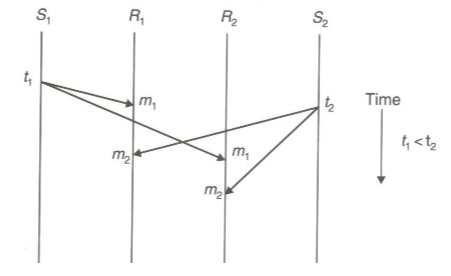
\includegraphics[width=0.7\linewidth]{figures/screenshot020}
\caption{Absolute ordering of many-to-many messages.}
\label{fig:screenshot020}
\end{figure}

\subsubsection{Consistent Ordering}
All messages are delivered to all receivers in the same order. However, this order may be different from the order in which the messages were originally sent.

A potential implementation of this follows: \begin{itemize}
\item Convert the communication to many-to-one and one-to-many by using a central node, called a \textit{sequencer}.
\item The sequencer will then receive messages from all of the sending nodes, assign a sequence number to each message, and then multicast it to all receiving nodes.
\end{itemize}

However, it is subject to a single point of failure and thus has poor reliability.

\begin{figure}[h]
\centering
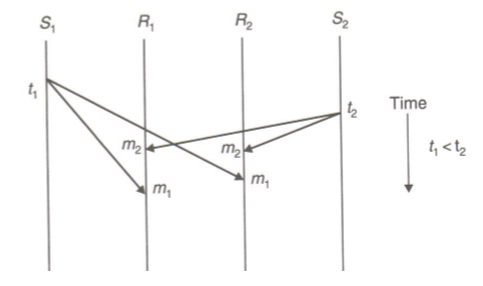
\includegraphics[width=0.7\linewidth]{figures/screenshot021}
\caption{Consistent ordering of many-to-many messages.}
\label{fig:screenshot021}
\end{figure}

\subsubsection{Causal Ordering}
\label{sssec:causalordering}
If the event of sending one message is causally related to the event of sending another message, the two messages are delivered to all receivers in the correct order.

Two message-sending events are said to be causally related if they are correlated by the \textit{happened-before} relation.

The happens-before relationship $a \rightarrow b$ is read "$a$ happens before $b$" and means that all processes agree that $a$ occurs, and then $b$ occurs afterwards. It is transitive, so $a \rightarrow b$ and $b \rightarrow c$ implies $a \rightarrow c$. It can be directly observed in two scenarios: \begin{enumerate}
\item If $a$ and $b$ are events in the same process, and $a$ occurs before $b$, then $a \rightarrow b$ is true.
\item If $a$ is the event of a message being sent by a process, and $b$ is the event of a message being received by another process, then $a \rightarrow b$ is true.
\end{enumerate}

An example of causal ordering can be found in CBCAST in the ISIS system.

\section{Remote Procedure Call (RPC)}
IPC in a distributed system is well-handled by a message-passing system, but any such IPC system is likely to be bespoke and will thus not be reusable across applications. As a result, a general IPC protocol was needed that could be reused; from this, the Remote Procedure Call (RPC) facility was created.

\begin{figure}
\centering
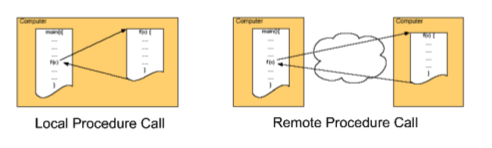
\includegraphics[width=0.7\linewidth]{figures/screenshot022}
\caption{Local procedure calls vs remote procedure calls}
\label{fig:screenshot022}
\end{figure}

Remote procedure calls are similar to local procedure calls (which invoke a procedure in a single process on a single host), but invoke a procedure on a remote machine (see \autoref{fig:screenshot022}). This allows them to offer a variety of features, including \begin{itemize}
\item simple call syntax
\item familiar syntax
\item specified well-defined interface
\item ease of use
\item generality
\item efficiency
\end{itemize}

The average RPC flow can be seen in \autoref{fig:screenshot023}.
\begin{figure}
\centering
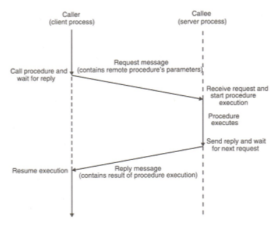
\includegraphics[width=0.7\linewidth]{figures/screenshot023}
\caption{A flow for the RPC model.}
\label{fig:screenshot023}
\end{figure}

To achieve semantic transparency (see \autoref{sssec:transparency}), RPC implementations use \textit{stubs}. A stub is a normal local procedure that translates the parameters from the client into a network-friendly format, and then submits them to the \textit{RPCRuntime}, responsible for sending it across to the network. This is illustrated in \autoref{fig:screenshot024}.

\begin{figure}
\centering
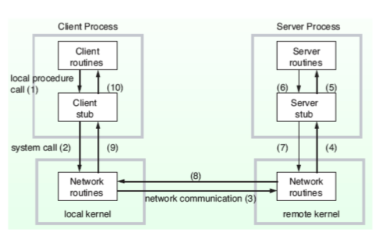
\includegraphics[width=0.7\linewidth]{figures/screenshot024}
\caption{RPC in detail.}
\label{fig:screenshot024}
\end{figure}

These stubs are typically generated from the interface definition (similar to a class definition in an object-oriented language) of the server routines using development tools. 

There are generally two types of RPC messages: call messages and reply messages. A call message is responsible for telling the receiver to call a particular procedure, while the reply message is the message from the receiver to the sender notifying them of the result of the call. This is illustrated in \autoref{fig:screenshot025}.

\begin{figure}
\centering
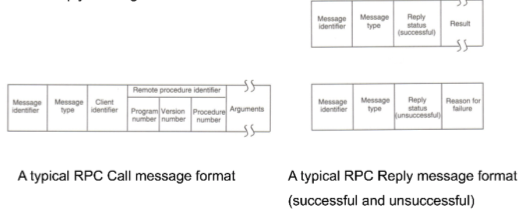
\includegraphics[width=0.7\linewidth]{figures/screenshot025}
\caption{RPC Call vs RPC Reply.}
\label{fig:screenshot025}
\end{figure}

\subsection{Parameter Handling}
Parameters may be passed to the stub in one of three ways: call-by-value, call-by-reference, and call-by-copy/restore.

In call-by-value, the value of the arguments are copied to the stack and passed to the procedure. The called procedure can modify its copy, but these modifications will not be propagated to the original value at the call site.

In call-by-reference, the memory addresses of the variables for the arguments are passed to the procedure. Changes made to the variables in the procedure will be propagated to the call site, as the call site variables \textit{are} the procedure variables.

In call-by-copy/restore, the values of the arguments are copied to the stack and are passed to the procedure (similar to call-by-value). However, when the procedure finishes executing, the values are copied back to the call site, providing similar behaviour to call-by-reference.

Call-by-value and call-by-copy/restore are relatively trivial to implement for RPCs, but call-by-reference is significantly harder as local memory addresses do not map to remote memory addresses. Implementation of call-by-reference is done by copying to the remote machine, using the copy's address, and then copying back at the end of execution (similar to call-by-copy/restore).

As parameters may have different encodings on different machines, it is important to encode them to a common format to transmit over the network. If a standard format is not used, both sides will have to encode and decode the message as appropriate. Alternatively, the message can be annotated with the format in use, and the receiving computer can decode the message knowing its format; but the receiver will need to be able to handle arbitrary formats.

\subsection{Variations}
There are multiple variations on RPCs. These are: \begin{itemize}
\item \textbf{Asynchronous RPC}: Typically, a RPC is synchronous; the calling code will wait for the call to finish executing on the remote machine. As this can lead to unnecessarily waiting, the remote machine can instead inform the calling code that it has accepted the request immediately. This dramatically reduces the amount of time spent waiting, as seen in \autoref{fig:screenshot026}. \begin{figure}
\centering
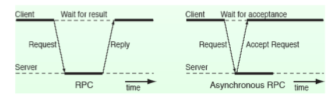
\includegraphics[width=0.7\linewidth]{figures/screenshot026}
\caption{Asynchronous RPC.}
\label{fig:screenshot026}
\end{figure}
\item \textbf{One-way RPC}: After sending the RPC to the remote machine, the calling code will immediately continue and not wait for a response.
\item \textbf{Callback RPC, Broadcast RPC, Batch-mode RPC, Lightweight RPC}: These are not explained.
\end{itemize}

\subsection{Optimisations For Better Performance}
To optimise RPC performance, the following can be investigated: \begin{itemize}
\item \textbf{Concurrent access to multiple servers}: A client can connect to multiple servers. To do this, it can use threads (where each thread can make independent RPCs to different servers), an early reply approach (where RPCs are made, and then the response is retrieved at a later stage), or a call buffering approach (where an intermediary is used to dispatch RPCs across clients and servers appropriately).
\item \textbf{Serving multiple requests simultaneously}: A server may be blocked on other resources while attending to a RPC, and will thus end up underutilised. To mitigate this, the server can handle other RPCs while waiting for the original resource to be freed. Threads can also help with this.
\item \textbf{Reducing per-call workload of servers}: Reducing the work associated with any given call will help performance in general.
\item \textbf{Reply caching of idempotent remote procedures}: See \autoref{ssec:idempotency}.
\item \textbf{Proper selection of timeout values}: If a RPC fails to respond, a long timeout could cause the client to stall for an extended period of time. A shorter timeout will reduce the delay before the client can choose its next course of action.
\item \textbf{Proper design of RPC protocol specification}: The RPC protocol should be designed for performance; otherwise, it may be unnecessarily inefficient.
\end{itemize}
